\documentclass[11pt,a4paper]{article}
\usepackage[T1]{fontenc}
\usepackage[utf8]{inputenc}
\usepackage{lmodern}
\usepackage{textcomp}
\usepackage[left=1.8cm,right=1.8cm,top=2.3cm,bottom=2.2cm,headheight=14pt,headsep=8pt]{geometry}
\usepackage{multicol}
\usepackage{xcolor}
\usepackage{fancyhdr}
\usepackage{graphicx}
\usepackage{array}
\usepackage{amsmath,amssymb}
\usepackage{setspace}
\usepackage{longtable}
\graphicspath{{../}}
\definecolor{ygreen}{RGB}{46,139,87}
\renewcommand{\normalsize}{\fontsize{10.9}{13.4}\selectfont}
\renewcommand{\familydefault}{\rmdefault}
\setlength{\parindent}{0pt}
\setlength{\columnsep}{0.8cm}
\setlength{\columnseprule}{0.4pt}
\setlength{\multicolsep}{3pt plus 1pt minus 1pt}
\renewcommand{\textsubscript}[1]{\ensuremath{_{\text{\fontsize{8}{8}\selectfont #1}}}}
\renewcommand{\textsuperscript}[1]{\ensuremath{^{\text{\fontsize{8}{8}\selectfont #1}}}}
\newcommand{\diqqat}[1]{\par\smallskip\noindent\textbf{Diqqat!} #1\par\medskip}
\newcommand{\javob}{\par\smallskip\noindent\textbf{Javob:} \rule[-2pt]{7.5cm}{0.4pt}\par\smallskip\noindent\textbf{Diqqat!} Javobingizni javoblar varaqasiga ko`chirib yozing.\par\medskip}
\pagestyle{fancy}
\fancyhf{}
\renewcommand{\headrulewidth}{0.4pt}
\fancyhead[L]{\textit{Milliy sertifikat 2026. Kimyo}}
\fancyhead[R]{12-variant}
\fancyfoot[L]{\fontsize{8}{9}\selectfont \textcopyright{} Colba maktabi, 2026}
\fancyfoot[C]{\thepage}
\fancypagestyle{first}{\fancyhf{}\renewcommand{\headrulewidth}{0pt}\fancyfoot[L]{\fontsize{8}{9}\selectfont \textcopyright{} Colba maktabi, 2026}\fancyfoot[C]{\thepage}}
\begin{document}
\normalsize
\thispagestyle{first}
\noindent\fcolorbox{ygreen}{white}{\parbox{\dimexpr\linewidth-2\fboxsep-2\fboxrule\relax}{%
\textbf{\fontsize{13}{15}\selectfont Nazorat testi}\ \textit{\fontsize{10}{12}\selectfont $\cdot$ Aralash test $\cdot$ 12-variant}\hfill
\begin{tabular}[t]{@{}r@{}}\textit{Milliy sertifikat 2026. Kimyo}\\ \textbf{\textit{\fontsize{8}{9}\selectfont Vaqt:}} \textit{\fontsize{10}{12}\selectfont 180 daqiqa}\end{tabular}}}
\par\medskip
\noindent\textit{Davriy jadvaldan foydalanish mumkin.}
\par\medskip
\begin{multicols}{2}
\noindent\textbf{1.} Rasmda davriy jadvalning bir qismi berilgan (\textit{X}, \textit{Y}, \textit{Z} --- noma'lum elementlar).
\begin{center}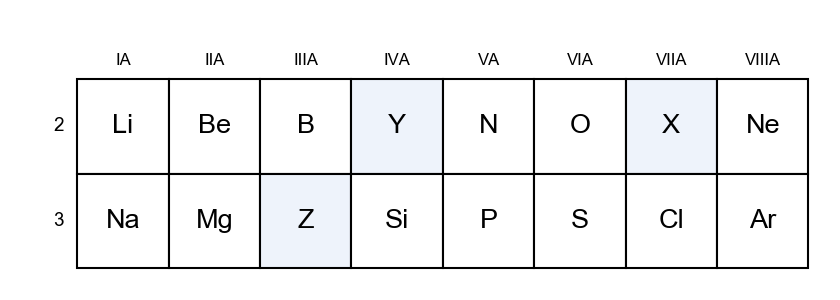
\includegraphics[width=0.86\linewidth]{rasmlar/gen/pt_259440.png}\end{center}
Qaysi elementlar metallar hisoblanadi?

\noindent A)~\textsl{\textit{Y}} \hfill B)~\textsl{\textit{Z}} \hfill C)~\textsl{\textit{X}} \hfill D)~\textsl{\textit{X}, \textit{Y}}\par
\vspace{4pt}
\noindent\textbf{2.} Jadvalda bog`lar hosil qiluvchi atomlarning elektrmanfiyliklari berilgan:
\begin{center}
\renewcommand{\arraystretch}{1.15}
\begin{tabular}{|c|c|c|}\hline
\textbf{Bog`} & \textbf{EM (1-atom)} & \textbf{EM (2-atom)} \\ \hline
H--Cl & 2,1 & 3 \\ \hline
H--O & 2,1 & 3,5 \\ \hline
H--F & 2,1 & 4 \\ \hline
C--O & 2,5 & 3,5 \\ \hline
\end{tabular}
\end{center}
Qaysi bog` eng qutbli (eng ko`p ionli xarakterga ega)?

\noindent A)~\textsl{H--Cl} \hfill B)~\textsl{H--O} \hfill C)~\textsl{C--O} \hfill D)~\textsl{H--F}\par
\vspace{4pt}
\noindent\textbf{3.} Quyidagi moddalarning qaysilarida ion bog` mavjud? 1) NaCl; 2) NH\textsubscript{4}Cl; 3) N\textsubscript{2}; 4) (NH\textsubscript{4})\textsubscript{2}SO\textsubscript{4}

\noindent A)~\textsl{1, 2, 4} \hfill B)~\textsl{2, 4} \hfill C)~\textsl{3, 4} \hfill D)~\textsl{1, 2, 3}\par
\vspace{4pt}
\noindent\textbf{4.} O\textsubscript{2} va CO\textsubscript{2} gazlari 3 : 4 hajmiy nisbatda aralashtirildi. Aralashmaning vodorodga nisbatan \textbf{zichligini aniqlang.}

\noindent A)~\textsl{38,86} \hfill B)~\textsl{20,43} \hfill C)~\textsl{19,43} \hfill D)~\textsl{19}\par
\vspace{4pt}
\noindent\textbf{5.} MgSO\textsubscript{4}$\cdot$7H\textsubscript{2}O kristallogidratida kristallizatsion suvning massa \textbf{ulushini (\%) aniqlang.}

\noindent A)~\textsl{48,8} \hfill B)~\textsl{25,6} \hfill C)~\textsl{105} \hfill D)~\textsl{51,2}\par
\vspace{4pt}
\noindent\textbf{6.} pH = 10 bo`lgan eritmada gidroksid ionlari konsentratsiyasi 10\textasciicircum{}($-$x) mol/l ga teng. x \textbf{ni aniqlang.}

\noindent A)~\textsl{4} \hfill B)~\textsl{10} \hfill C)~\textsl{5} \hfill D)~\textsl{9}\par
\vspace{4pt}
\noindent\textbf{7.} Tabiiy elementning ikki izotopi: \textsuperscript{10}B (20\%) va \textsuperscript{11}B (80\%). Elementning o`rtacha nisbiy atom \textbf{massasini aniqlang.}

\noindent A)~\textsl{10,8} \hfill B)~\textsl{10,5} \hfill C)~\textsl{10,2} \hfill D)~\textsl{10}\par
\vspace{4pt}
\noindent\textbf{8.} Quruq havo tarkibi diagrammada keltirilgan.
\begin{center}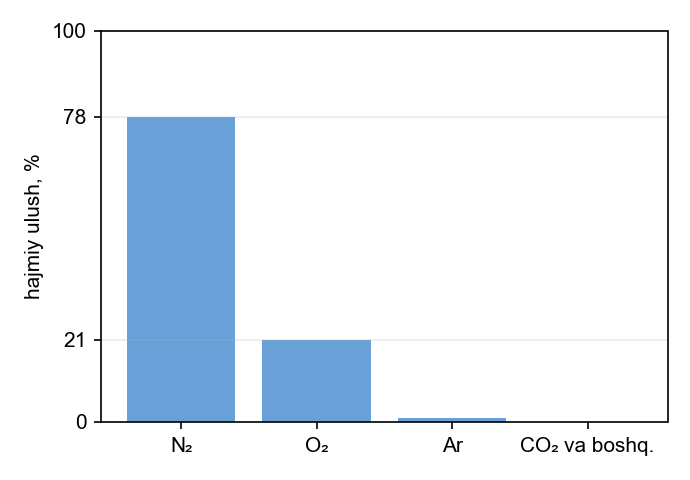
\includegraphics[width=0.86\linewidth]{rasmlar/gen/ai_v12_0.png}\end{center}
100 l (n.sh.) havo tarkibidagi kislorod \textbf{hajmini (l) toping.}

\noindent A)~\textsl{78} \hfill B)~\textsl{42} \hfill C)~\textsl{21} \hfill D)~\textsl{10,5}\par
\vspace{4pt}
\noindent\textbf{9.} 12,5 g CuSO\textsubscript{4}$\cdot$5H\textsubscript{2}O 100 g suvda eritildi. Eritmadagi tuzning massa \textbf{ulushini (\%) aniqlang.}

\noindent A)~\textsl{8} \hfill B)~\textsl{7,11} \hfill C)~\textsl{11,11} \hfill D)~\textsl{14,22}\par
\vspace{4pt}
\noindent\textbf{10.} 30 l CH\textsubscript{4} va 120 l O\textsubscript{2} aralashmasi CH\textsubscript{4} + 2O\textsubscript{2} $\to$ CO\textsubscript{2} + 2H\textsubscript{2}O tenglama bo`yicha to`liq reaksiyaga kirishdi (reaksiyadan so`ng suv suyuq holatda; gazlar bir xil sharoitda o`lchandi). Reaksiyadan so`ng ortib qolgan O\textsubscript{2} ning \textbf{hajmini (l) aniqlang.}

\noindent A)~\textsl{60} \hfill B)~\textsl{120} \hfill C)~\textsl{30} \hfill D)~\textsl{90}\par
\vspace{4pt}
\noindent\textbf{11.} Jadvalda metall plastinkalarning tuz eritmalariga tushirilishidagi kuzatuvlar berilgan (``+'' -- metall ajraladi, reaksiya boradi; ``$-$'' -- reaksiya bormaydi):
\begin{center}
\renewcommand{\arraystretch}{1.15}
\begin{tabular}{|c|c|c|c|}\hline
\textbf{Metall} & \textbf{FeSO\textsubscript{4} eritmasi} & \textbf{AgNO\textsubscript{3} eritmasi} & \textbf{ZnSO\textsubscript{4} eritmasi} \\ \hline
Mg & + & + & + \\ \hline
Cu & $-$ & + & $-$ \\ \hline
Fe & $-$ & + & $-$ \\ \hline
\end{tabular}
\end{center}
Ushbu metallardan qaysi biri eng faol?

\noindent A)~\textsl{Mg} \hfill B)~\textsl{Cu} \hfill C)~\textsl{Fe} \hfill D)~\textsl{Zn}\par
\vspace{4pt}
\noindent\textbf{12.} Faqat oksidlovchi bo`la oladigan \textbf{ionlarni aniqlang}: 1) Zn\textsuperscript{2+}; 2) Fe\textsuperscript{2+}; 3) Fe\textsuperscript{3+}; 4) Al\textsuperscript{3+}

\noindent A)~\textsl{1, 4} \hfill B)~\textsl{2, 4} \hfill C)~\textsl{3} \hfill D)~\textsl{4}\par
\vspace{4pt}
\noindent\textbf{13.} 35-tartib raqamli elementning barcha elektronlaridan nechtasining spin kvant soni m\_s = +$\frac{1}{2}$ ga teng (Hund qoidasi bo`yicha to`ldirilgan holat)?

\noindent A)~\textsl{19} \hfill B)~\textsl{17} \hfill C)~\textsl{20} \hfill D)~\textsl{18}\par
\vspace{4pt}
\noindent\textbf{14.} Qaysi juftliklar o`zaro reaksiyaga kirishadi? 1) Fe va HCl; 2) Fe\textsubscript{2}O\textsubscript{3} va H\textsubscript{2}O; 3) CuSO\textsubscript{4} va NaOH; 4) CuO va H\textsubscript{2}

\noindent A)~\textsl{1, 2, 4} \hfill B)~\textsl{2, 3} \hfill C)~\textsl{1, 3} \hfill D)~\textsl{1, 3, 4}\par
\vspace{4pt}
\noindent\textbf{15.} NaNO\textsubscript{3} qizdirilganda qanday moddalar hosil bo`ladi?

\noindent\begin{tabular}{@{}p{0.47\linewidth}@{}p{0.47\linewidth}@{}}
A)~\textsl{KNO\textsubscript{2} va O\textsubscript{2}} & B)~\textsl{NaNO\textsubscript{2} va O\textsubscript{2}} \\
C)~\textsl{ZnO, NO\textsubscript{2} va O\textsubscript{2}} & D)~\textsl{Ag, NO\textsubscript{2} va O\textsubscript{2}} \\
\end{tabular}\par
\vspace{4pt}
\noindent\textbf{16.} 2Mg + CO\textsubscript{2} $\to$ 2MgO + C jarayoni uchun 4,48 l (n.sh.) CO\textsubscript{2} olingan. MgO \textbf{miqdorini (mol) aniqlang.}

\noindent A)~\textsl{0,1} \hfill B)~\textsl{0,8} \hfill C)~\textsl{0,2} \hfill D)~\textsl{0,4}\par
\vspace{4pt}
\noindent\textbf{17.} Reaksiya tenglamasi: MnO\textsubscript{2} + 4HCl $\to$ MnCl\textsubscript{2} + Cl\textsubscript{2} + 2H\textsubscript{2}O. Reaksiyaga 22,4 l (n.sh.) HCl kirishdi. MnCl\textsubscript{2} \textbf{massasini (g) hisoblang.}

\noindent A)~\textsl{504} \hfill B)~\textsl{31,5} \hfill C)~\textsl{63} \hfill D)~\textsl{15,75}\par
\vspace{4pt}
\noindent\textbf{18.} Na\textsubscript{2}O + H\textsubscript{2}O $\to$ 2NaOH reaksiyasida 6,2 g Na\textsubscript{2}O ishtirok etdi (unum 90\%). NaOH \textbf{massasini (g) toping.}

\noindent A)~\textsl{2} \hfill B)~\textsl{7,2} \hfill C)~\textsl{14,4} \hfill D)~\textsl{3,6}\par
\vspace{4pt}
\noindent\textbf{19.} Alyuminiy va magniy dan iborat 10,2 g aralashma mo`l xlorid kislotada eritilganda 11,2 l (n.sh.) vodorod ajraldi. Aralashmadagi alyuminiyning massa \textbf{ulushini (\%) aniqlang.}

\noindent A)~\textsl{52,9} \hfill B)~\textsl{47,1} \hfill C)~\textsl{26,5} \hfill D)~\textsl{5,4}\par
\vspace{4pt}
\noindent\textbf{20.} Uglevodorodning 4,4 g massasi yondirilganda 13,2 g CO\textsubscript{2} va 7,2 g H\textsubscript{2}O hosil bo`ldi. Uglevodorod molekulasidagi uglerod atomlari \textbf{sonini toping} (M = 44 g/mol).

\noindent A)~\textsl{4} \hfill B)~\textsl{2} \hfill C)~\textsl{8} \hfill D)~\textsl{3}\par
\vspace{4pt}
\noindent\textbf{21.} 23 g etil spirtidan Lebedev usuli bilan (80\% unum) butadiyen-1,3 olindi (2C\textsubscript{2}H\textsubscript{5}OH $\to$ C\textsubscript{4}H\textsubscript{6} + H\textsubscript{2} + 2H\textsubscript{2}O). Butadiyen \textbf{massasini (g) aniqlang.}

\noindent A)~\textsl{10,8} \hfill B)~\textsl{21,6} \hfill C)~\textsl{13,5} \hfill D)~\textsl{23}\par
\vspace{4pt}
\noindent\textbf{22.} 26 g C\textsubscript{2}H\textsubscript{2} dan quyidagi ikki bosqichda CH\textsubscript{3}COOH olinadi: 1) C\textsubscript{2}H\textsubscript{2} + H\textsubscript{2}O $\to$ CH\textsubscript{3}CHO (unum 60\%); 2) CH\textsubscript{3}CHO + 2Ag\textsubscript{2}O $\to$ CH\textsubscript{3}COOH + 4Ag (unum 50\%). Oxirgi mahsulot CH\textsubscript{3}COOH ning \textbf{massasini (g) toping.}

\noindent A)~\textsl{30} \hfill B)~\textsl{36} \hfill C)~\textsl{18} \hfill D)~\textsl{60}\par
\vspace{4pt}
\noindent\textbf{23.} C\textsubscript{6}H\textsubscript{12}O\textsubscript{6} (bijg`ish) reaksiyasi natijasida qaysi organik modda hosil bo`ladi?

\noindent A)~\textsl{etilen} \hfill B)~\textsl{metan} \hfill C)~\textsl{etanol} \hfill D)~\textsl{benzol}\par
\vspace{4pt}
\noindent\textbf{24.} Aldegid va ketonlar haqida qaysi fikrlar to`g`ri? 1) Ketonlar kuchsiz oksidlovchilar bilan oksidlanmaydi; 2) Aldegidlar "kumush ko`zgu" reaksiyasini beradi; 3) Aseton suvda erimaydi; 4) Aseton Cu(OH)\textsubscript{2} ni qaytaradi

\noindent A)~\textsl{2, 3, 4} \hfill B)~\textsl{1, 2} \hfill C)~\textsl{1, 2, 3} \hfill D)~\textsl{2, 4}\par
\vspace{4pt}
\noindent\textbf{25.} 12 g sirka kislota ni neytrallash uchun 10\% li NaOH eritmasidan necha gramm kerak?

\noindent A)~\textsl{8} \hfill B)~\textsl{80} \hfill C)~\textsl{40} \hfill D)~\textsl{120}\par
\vspace{4pt}
\noindent\textbf{26.} Murakkab efirlar va yog`lar haqida qaysi fikrlar to`g`ri? 1) Yog`lar glitserin va yuqori yog` kislotalarning murakkab efirlari; 2) Sovun --- yuqori yog` kislotalarning natriyli tuzi; 3) Dietil efir spirtdan yuqori haroratda qaynaydi; 4) Efirlanish reaksiyasi qaytmas

\noindent A)~\textsl{1, 2, 3} \hfill B)~\textsl{1} \hfill C)~\textsl{1, 2} \hfill D)~\textsl{2, 3}\par
\vspace{4pt}
\noindent\textbf{27.} 34,2 g saxaroza gidrolizlanganda necha gramm glyukoza hosil bo`ladi?

\noindent A)~\textsl{34,2} \hfill B)~\textsl{36} \hfill C)~\textsl{9} \hfill D)~\textsl{18}\par
\vspace{4pt}
\noindent\textbf{28.} Aminlar, aminokislotalar va oqsillar haqida qaysi fikrlar to`g`ri? 1) Aminokislotalar faqat kislotali xossaga ega; 2) Glitsin optik faol; 3) Dipeptidda 2 ta peptid bog` bor; 4) Nitrobenzoldan anilin Zinin reaksiyasi bilan olinadi

\noindent A)~\textsl{3} \hfill B)~\textsl{1} \hfill C)~\textsl{4} \hfill D)~\textsl{1, 4}\par
\vspace{4pt}
\noindent\textbf{29.} Yuqori molekulyar birikmalar haqida qaysi fikrlar to`g`ri? 1) Tabiiy kauchuk -- sis-1,4-poliizopren; 2) Fenolformaldegid smola polikondensatsiya mahsuloti; 3) Polimerning M = zveno M $\cdot$ polimerlanish darajasi; 4) Kapron poliamid tola

\noindent\begin{tabular}{@{}p{0.47\linewidth}@{}p{0.47\linewidth}@{}}
A)~\textsl{1, 2, 3} & B)~\textsl{1, 2, 3, 4} \\
C)~\textsl{1, 2, 4} & D)~\textsl{2, 3, 4} \\
\end{tabular}\par
\vspace{4pt}
\noindent\textbf{30.} Kimyo laboratoriyasida ishlash qoidalari haqida qaysi fikrlar to`g`ri? 1) Probirka qizdirilganda og`zi odamga qaratilmaydi; 2) Reaktivlarni tatib ko`rish mumkin; 3) Kuygan joy ko`p suv bilan yuviladi; 4) Ishqor teriga tushsa, qo`l suv bilan yuviladi

\noindent A)~\textsl{3, 4} \hfill B)~\textsl{2, 4} \hfill C)~\textsl{1, 3, 4} \hfill D)~\textsl{1, 3}\par
\vspace{4pt}
\noindent\textbf{31.} Fenolftalein indikatori ishqoriy muhitda qanday rang beradi?
\noindent A)~\textsl{qizil}\par
\noindent B)~\textsl{ko`k}\par
\noindent C)~\textsl{sariq}\par
\noindent D)~\textsl{malina rangga kiradi (pushti)}\par
\vspace{4pt}
\noindent\textbf{32.} Rasmda alanganing 2 raqami bilan ko`rsatilgan qismi qanday xususiyatga ega?
\begin{center}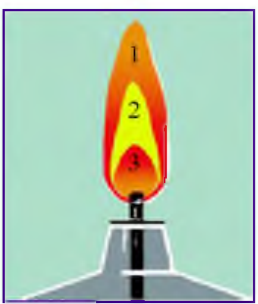
\includegraphics[width=0.86\linewidth]{rasmlar/darslik/d_alanga.png}\end{center}
\noindent A)~\textsl{rangsiz va sovuq qism}\par
\noindent B)~\textsl{chetlari xira, eng issiq qism}\par
\noindent C)~\textsl{ravshan, issiq qism}\par
\noindent D)~\textsl{juda xira, issiq bo`lmagan qism   ---}\par
\vspace{4pt}
\end{multicols}
\medskip
\noindent\setlength{\fboxsep}{0pt}\fbox{\begin{tabular}{p{0.74\linewidth}|p{0.2\linewidth}}
\parbox[t]{0.72\linewidth}{\vspace{3pt}\textbf{Topshiriqlar (33--35) va javob variant (A--F)larini o`zaro to`g`ri moslashtiring.} CuO va Fe\textsubscript{2}O\textsubscript{3} dan iborat 48 g aralashma qizdirilib, CO oqimida to`liq qaytarildi; qoldiq (metallar) massasi 35,2 g.
\vspace{3pt}} & \parbox[t]{0.19\linewidth}{\vspace{3pt}A~\textsl{12,8}\\[3pt]
B~\textsl{35,2}\\[3pt]
C~\textsl{8}\\[3pt]
D~\textsl{21,5}\\[3pt]
E~\textsl{32,26}\\[3pt]
F~\textsl{16}}\\ \hline
\parbox[t]{0.72\linewidth}{\vspace{2pt}\textbf{33. Aralashmadagi CuO massasini (g) aniqlang.}\vspace{2pt}} & \\ \hline
\parbox[t]{0.72\linewidth}{\vspace{2pt}\textbf{34. Qaytarish uchun (20\% ortiqcha olingan) sarflangan CO hajmini (l, n.sh.) aniqlang.}\vspace{2pt}} & \\ \hline
\parbox[t]{0.72\linewidth}{\vspace{2pt}\textbf{35. Qaytarish natijasida hosil bo`lgan CO\textsubscript{2} massasini (g) aniqlang.}\vspace{2pt}} & 
\end{tabular}}
\par\bigskip
\noindent\textbf{36.} C + HNO\textsubscript{3} $\to$ CO\textsubscript{2} + NO\textsubscript{2} + H\textsubscript{2}O reaksiya tenglamasini tenglang. Reagentlar (chap qism) koeffitsiyentlari \textbf{yig`indisini toping.}
\javob
\noindent\textbf{37.} CuCl\textsubscript{2} eritmasi inert elektrodlar yordamida 4 A tok kuchi bilan 3860 s elektroliz qilindi. Anodda ajralgan Cl\textsubscript{2} hajmi (l, n.sh.) \textbf{ni toping.}
\javob
\noindent\textbf{38.} Al, Fe va Cu dan iborat aralashma mo`l NaOH eritmasi bilan ta'sirlashganda 3,36 l (n.sh.) vodorod ajraldi; xuddi shunday massadagi aralashma mo`l HCl bilan ta'sirlashganda 7,84 l (n.sh.) vodorod ajraldi, erimay qolgan qoldiq (mis) massasi 3,2 g. Aralashmaning dastlabki \textbf{massasini (g) toping.}
\javob
\noindent\textbf{39.} Uglevodorodning 8,4 g massasi yondirilganda 26,4 g CO\textsubscript{2} va 10,8 g H\textsubscript{2}O hosil bo`ldi. Uglevodorodning molyar \textbf{massasini (g/mol) aniqlang.}
\javob
\noindent\textbf{40.} Etilen dan olingan polimerning molyar massasi 56000 g/mol. Polimerlanish \textbf{darajasini aniqlang.}
\javob
\par\bigskip\begin{center}\textbf{\fontsize{13}{15}\selectfont YOZMA ISH}\end{center}
\noindent\textbf{41.} \textbf{Topshiriqni bajarish jarayonida barcha reaksiya tenglamalarini yozing. Miqdoriy va arifmetik hisoblashlarni (unga asos bo`lgan usul yoki formulani ko`rsatgan holda) uzviy ketma-ketlikda bajaring.}\par\smallskip
Hajmi 1 l bo`lgan idishga 0,8 mol SO\textsubscript{2} va ma'lum miqdorda O\textsubscript{2} solindi hamda katalizator ishtirokida qizdirildi: 2SO\textsubscript{2} + O\textsubscript{2} $\rightleftarrows$ 2SO\textsubscript{3}. Muvozanat qaror topganda idishda SO\textsubscript{2}, O\textsubscript{2} va SO\textsubscript{3} ning mol nisbati 1 : 1 : 3 bo`ldi.\par
Hosil bo`lgan SO\textsubscript{3} ning hammasi 100 g 49\% li H\textsubscript{2}SO\textsubscript{4} eritmasiga yuttirildi (oleum hosil bo`lmadi, SO\textsubscript{3} to`liq suv bilan reaksiyaga kirishdi). Olingan eritmaga mo`l BaCl\textsubscript{2} eritmasi qo`shildi.\par
\noindent 1)O\textsubscript{2} ning boshlang`ich miqdorini (mol) va muvozanat konstantasini (K) hisoblang.\par
\noindent 2)SO\textsubscript{2} ning necha foizi reaksiyaga kirishgan? Muvozanatda SO\textsubscript{3} ning hajmiy ulushini (\%) ham toping.\par
\noindent 3)SO\textsubscript{3} yuttirilgandan keyingi eritmada H\textsubscript{2}SO\textsubscript{4} ning massa ulushini (\%) aniqlang.\par
\noindent 4)BaCl\textsubscript{2} qo`shilganda hosil bo`lgan cho`kma massasini (g) toping. BaCl\textsubscript{2} sarfini (g) ham toping.\par
\noindent 5)Doimiy haroratda idish hajmi 2 marta kamaytirilsa (v = k$\cdot$[SO\textsubscript{2}]\textsuperscript{2}$\cdot$[O\textsubscript{2}]), to`g`ri reaksiya tezligi necha marta o`zgaradi? Shuningdek muvozanatda umumiy bosimning boshlang`ich bosimga nisbatini (T = const) toping.\par
\diqqat{Mazkur topshiriq kengaytirilgan javobni talab etib, uning yechilish usuli va shu usul asosidagi barcha hisoblash amallari javoblar varaqasida aks etishi lozim.}
\noindent\textbf{42.} Reaksiya tenglamalarini tugallang va tenglang. Hosil bo`lgan organik moddalarning tuzilish formulalarini yozing va ularni nomlang.\par
\noindent 1)HCOOH + Ag\textsubscript{2}O $\xrightarrow{\text{NH\textsubscript{3}, t}}$\par
\noindent 2)(C\textsubscript{17}H\textsubscript{35}COO)\textsubscript{3}C\textsubscript{3}H\textsubscript{5} + NaOH $\to$\par
\noindent 3)CH\textsubscript{3}--CH=CH\textsubscript{2} + HBr $\to$\par
\noindent 4)C\textsubscript{6}H\textsubscript{12}O\textsubscript{6} $\xrightarrow{\text{spirtli bijg`ish}}$\par
\noindent 5)C\textsubscript{2}H\textsubscript{5}Br + KOH(spirtli) $\to$\par
\noindent 6)CH\textsubscript{3}--CH(OH)--CH\textsubscript{3} + CuO $\xrightarrow{\text{t}}$\par
\noindent 7)n CH\textsubscript{2}=CH\textsubscript{2} $\to$\par
\diqqat{Mazkur topshiriq kengaytirilgan javobni talab etib, uning yechilish usuli va shu usul asosidagi barcha hisoblash amallari javoblar varaqasida aks etishi lozim.}
\noindent\textbf{43.} \textbf{Topshiriqni bajarish jarayonida barcha reaksiya tenglamalarini yozing. Miqdoriy va arifmetik hisoblashlarni (unga asos bo`lgan usul yoki formulani ko`rsatgan holda) uzviy ketma-ketlikda bajaring.}\par\smallskip
Alyuminiy, magniy va misdan iborat 8,3 g aralashma mo`l NaOH eritmasi bilan reaksiyaga kirishganda 3,36 l (n.sh.) vodorod ajraldi. Xuddi shunday tarkibli 8,3 g aralashma mo`l xlorid kislota bilan reaksiyaga kirishganda esa 5,6 l (n.sh.) vodorod ajraldi.\par
\noindent 1)Aralashmadagi har bir metallning massasini (g) va massa ulushini (\%) aniqlang (reaksiya tenglamalarini yozing).\par
\noindent 2)Xlorid kislota bilan reaksiyadan keyin qolgan qoldiq konsentrlangan HNO\textsubscript{3} da to`liq eritildi. Ajralgan gazning hajmini (l, n.sh.) hisoblang.\par
\noindent 3)Xlorid kislota bilan olingan eritmaga mo`l NaOH qo`shildi, cho`kma ajratib olinib, quritildi. Cho`kma massasini (g) toping.\par
\noindent 4)Hosil bo`lgan Cu(NO\textsubscript{3})\textsubscript{2} eritmasi bug`latilib, quruq tuz qizdirilganda hosil bo`ladigan qattiq qoldiq massasini (g) va gazlar aralashmasining hajmini (l, n.sh.) aniqlang.\par
\noindent 5)Ushbu aralashma (butun massasi) to`liq reaksiyaga kirishishi uchun 20\% li HCl eritmasidan necha gramm kerak (mis reaksiyaga kirishmaydi)?\par
\diqqat{Mazkur topshiriq kengaytirilgan javobni talab etib, uning yechilish usuli va shu usul asosidagi barcha hisoblash amallari javoblar varaqasida aks etishi lozim.}
\newpage
\noindent\textbf{\fontsize{13}{15}\selectfont Nazorat testi}\ \textit{$\cdot$ 12-variant}\hfill \textbf{Javoblar kaliti}\par\smallskip\hrule\smallskip
\textit{Faqat o`qituvchi uchun.}\par\medskip
\noindent\textbf{1--32-savollar}\par\smallskip
\noindent\begin{tabular}{|c|c|c|c|c|c|c|c|c|c|c|c|c|c|c|c|}\hline
\textbf{1} & \textbf{2} & \textbf{3} & \textbf{4} & \textbf{5} & \textbf{6} & \textbf{7} & \textbf{8} & \textbf{9} & \textbf{10} & \textbf{11} & \textbf{12} & \textbf{13} & \textbf{14} & \textbf{15} & \textbf{16}\\\hline
\textsl{B} & \textsl{D} & \textsl{A} & \textsl{C} & \textsl{D} & \textsl{A} & \textsl{A} & \textsl{C} & \textsl{B} & \textsl{A} & \textsl{A} & \textsl{A} & \textsl{D} & \textsl{D} & \textsl{B} & \textsl{D}\\\hline
\textbf{17} & \textbf{18} & \textbf{19} & \textbf{20} & \textbf{21} & \textbf{22} & \textbf{23} & \textbf{24} & \textbf{25} & \textbf{26} & \textbf{27} & \textbf{28} & \textbf{29} & \textbf{30} & \textbf{31} & \textbf{32}\\\hline
\textsl{B} & \textsl{B} & \textsl{A} & \textsl{D} & \textsl{A} & \textsl{C} & \textsl{C} & \textsl{B} & \textsl{B} & \textsl{C} & \textsl{D} & \textsl{C} & \textsl{B} & \textsl{C} & \textsl{D} & \textsl{C}\\\hline
\end{tabular}\par\medskip
\noindent\textbf{33--35-savollar}\par\smallskip
\noindent\begin{tabular}{|c|c|c|}\hline \textbf{No} & \textbf{Javob} & \textbf{Qiymat}\\\hline
33 & \textsl{F} & 16\\\hline
34 & \textsl{D} & 21,5\\\hline
35 & \textsl{B} & 35,2\\\hline
\end{tabular}\par\medskip
\noindent\textbf{36--40-savollar}\par\smallskip
\noindent\begin{tabular}{|c|c|}\hline \textbf{No} & \textbf{To`g`ri javob}\\\hline
36 & 5\\\hline
37 & 1,792\\\hline
38 & 17,1\\\hline
39 & 42\\\hline
40 & 2000\\\hline
\end{tabular}\par\medskip
\noindent\textbf{41--43-topshiriqlar: qisqa yechim}\par\smallskip
\noindent\textbf{41-topshiriq.}\par
\noindent 1) SO\textsubscript{2} : O\textsubscript{2} : SO\textsubscript{3} = 1 : 1 : 3 $\to$ SO\textsubscript{2} = x, SO\textsubscript{3} = 3x; x + 3x = 0,8 $\to$ x = 0,2 mol. O\textsubscript{2} sarfi 1,5x = 0,3; O\textsubscript{2} boshlang`ich = 0,2 + 0,3 = \textbf{0,5 mol}; [SO\textsubscript{2}] = 0,2, [O\textsubscript{2}] = 0,2, [SO\textsubscript{3}] = 0,6 $\to$ K = [SO\textsubscript{3}]\textsuperscript{2}/([SO\textsubscript{2}]\textsuperscript{2}$\cdot$[O\textsubscript{2}]) = \textbf{45}\par
\noindent 2) $\alpha$ = 3x/4x = \textbf{75\%}; $\varphi$(SO\textsubscript{3}) = 3x/5x = \textbf{60\%}\par
\noindent 3) SO\textsubscript{3} = 0,6 mol = 48 g; 100 g 49\% li eritmada H\textsubscript{2}SO\textsubscript{4} 49 g; SO\textsubscript{3} + H\textsubscript{2}O $\to$ H\textsubscript{2}SO\textsubscript{4}: +58,8 g; jami 107,8 g; eritma 148 g $\to$ $\omega$ = \textbf{72,84\%}\par
\noindent 4) H\textsubscript{2}SO\textsubscript{4} + BaCl\textsubscript{2} $\to$ BaSO\textsubscript{4}$\downarrow$ + 2HCl: n(H\textsubscript{2}SO\textsubscript{4}) = 1,1 mol $\to$ BaSO\textsubscript{4} 256,3 g = \textbf{256,3 g}; m(BaCl\textsubscript{2}) = 1,1$\cdot$208 = \textbf{228,8 g}\par
\noindent 5) Hajm 2 marta kamayganda konsentratsiyalar 2 marta ortadi: v\textsubscript{2}/v\textsubscript{1} = 2\textsuperscript{2} $\cdot$ 2 = \textbf{8 marta ortadi}; n(muv.)/n(bosh.) = 5x/6,5x = \textbf{0,77}\par
\noindent Jami: M 15 + A 10 = 25 ball.\par
\noindent\textbf{42-topshiriq.}\par
\noindent 1) HCOOH + Ag\textsubscript{2}O $\xrightarrow{\text{NH\textsubscript{3}, t}}$ CO\textsubscript{2} + H\textsubscript{2}O + 2Ag$\downarrow$ --- karbonat angidrid (3 ball)\par
\noindent 2) (C\textsubscript{17}H\textsubscript{35}COO)\textsubscript{3}C\textsubscript{3}H\textsubscript{5} + NaOH $\to$ 3C\textsubscript{17}H\textsubscript{35}COONa + C\textsubscript{3}H\textsubscript{5}(OH)\textsubscript{3} --- natriy stearat (sovun) va glitserin (4 ball)\par
\noindent 3) CH\textsubscript{3}--CH=CH\textsubscript{2} + HBr $\to$ CH\textsubscript{3}--CHBr--CH\textsubscript{3} --- 2-brompropan (Markovnikov) (3 ball)\par
\noindent 4) C\textsubscript{6}H\textsubscript{12}O\textsubscript{6} $\xrightarrow{\text{spirtli bijg`ish}}$ 2C\textsubscript{2}H\textsubscript{5}OH + 2CO\textsubscript{2} --- etanol (3 ball)\par
\noindent 5) C\textsubscript{2}H\textsubscript{5}Br + KOH(spirtli) $\to$ CH\textsubscript{2}=CH\textsubscript{2} + KBr + H\textsubscript{2}O --- etilen (4 ball)\par
\noindent 6) CH\textsubscript{3}--CH(OH)--CH\textsubscript{3} + CuO $\xrightarrow{\text{t}}$ CH\textsubscript{3}COCH\textsubscript{3} + Cu + H\textsubscript{2}O --- propanon (4 ball)\par
\noindent 7) n CH\textsubscript{2}=CH\textsubscript{2} $\to$ (--CH\textsubscript{2}--CH\textsubscript{2}--)n --- polietilen (4 ball)\par
\noindent Jami 25 ball.\par
\noindent\textbf{43-topshiriq.}\par
\noindent 1) NaOH bilan faqat Al reaksiyaga kirishadi: n(Al) = 0,1 mol = 2,7 g; HCl bilan: n(Mg) = 0,1 mol = 2,4 g; Cu = 3,2 g. $\omega$: Al 32,5\%, Mg 28,9\%, Cu 38,6\%\par
\noindent 2) Cu + 4HNO\textsubscript{3}(kons.) $\to$ Cu(NO\textsubscript{3})\textsubscript{2} + 2NO\textsubscript{2} + 2H\textsubscript{2}O: NO\textsubscript{2} 0,1 mol $\to$ \textbf{2,24 l}\par
\noindent 3) MgCl\textsubscript{2} + 2NaOH $\to$ Mg(OH)\textsubscript{2}$\downarrow$ + 2NaCl; Mg(OH)\textsubscript{2} o`zgarmaydi: \textbf{5,8 g}\par
\noindent 4) 2Cu(NO\textsubscript{3})\textsubscript{2} $\to$ 2CuO + 4NO\textsubscript{2} + O\textsubscript{2}: CuO 0,05 mol = \textbf{4 g}; gazlar 0,125 mol $\to$ \textbf{2,8 l}\par
\noindent 5) n(HCl) = 2$\cdot$(0,15 + 0,1) = 0,25 mol $\to$ m = 0,5$\cdot$36,5/0,2 = \textbf{91,2 g}\par
\noindent Jami: M 15 + A 10 = 25 ball.\par
\par\bigskip\noindent\textbf{Mavzular taqsimoti}\par\smallskip
{\small\noindent\begin{longtable}{|c|p{7.2cm}|p{5.4cm}|c|}\hline \textbf{No} & \textbf{Mavzu} & \textbf{Tekshiriladigan ko`nikma} & \textbf{Ball}\\\hline
1 & 8-sinf (metallar va metallmaslar, jadval) & Rasm bo`yicha tahlil & 1\\\hline
2 & 8-sinf (kimyoviy bog`lanish turlari, jadval) & Jadval tahlili & 1\\\hline
3 & 8-sinf; Tirkashev II bob (kimyoviy bog`lanish) & Bilim va tushunish & 1\\\hline
4 & 11-sinf (D) & Hisoblash va masala yechish & 1\\\hline
5 & 7-sinf; Tirkashev (kristallogidrat) & Hisoblash va masala yechish & 1\\\hline
6 & Tirkashev IV bob (suvning ion ko`paytmasi) & Hisoblash va masala yechish & 1\\\hline
7 & 8-sinf (izotoplar) & Hisoblash va masala yechish & 1\\\hline
8 & 8-sinf (havo tarkibi, diagramma) & Grafik tahlili & 1\\\hline
9 & Tirkashev III bob (kristallogidrat) & Hisoblash va masala yechish & 1\\\hline
10 & 8-sinf (Gey-Lyussak qonuni) & Hisoblash va masala yechish & 1\\\hline
11 & Tirkashev \textit{V} bob (kuchlanish qatori, jadval) & Jadval tahlili & 1\\\hline
12 & Tirkashev \textit{V} bob; 11-sinf 7-bob & Bilim va tushunish & 1\\\hline
13 & Tirkashev I bob (kvant sonlari) & Bilim va tushunish & 1\\\hline
14 & 9-sinf; Tashev (anorganik birikmalar xossalari) & Bilim va tushunish & 1\\\hline
15 & Tashev (nitratlar) & Bilim va tushunish & 1\\\hline
16 & 9-sinf; Tirkashev (P/C/Si, hisob) & Hisoblash va masala yechish & 1\\\hline
17 & 9-sinf; Tirkashev (galogenlar, hisob) & Hisoblash va masala yechish & 1\\\hline
18 & 9-sinf; Tirkashev (IA metallar, hisob) & Hisoblash va masala yechish & 1\\\hline
19 & 9-sinf (Al, Mg, Ca) & Hisoblash va masala yechish & 1\\\hline
20 & 10-sinf (formulani aniqlash) & Hisoblash va masala yechish & 1\\\hline
21 & 10-sinf \S{}14; Abdusamatov (Lebedev) & Hisoblash va masala yechish & 1\\\hline
22 & 10-sinf (ikki bosqichli hisob) & Hisoblash va masala yechish & 1\\\hline
23 & 10-sinf (olinish usullari) & Bilim va tushunish & 1\\\hline
24 & 10-sinf (mavzuga oid paragraflar); Abdusamatov & Bilim va tushunish & 1\\\hline
25 & 10-sinf \S{}26 & Hisoblash va masala yechish & 1\\\hline
26 & 10-sinf (mavzuga oid paragraflar); Abdusamatov & Bilim va tushunish & 1\\\hline
27 & 10-sinf \S{}31 & Hisoblash va masala yechish & 1\\\hline
28 & 10-sinf (mavzuga oid paragraflar); Abdusamatov & Bilim va tushunish & 1\\\hline
29 & 10-sinf (mavzuga oid paragraflar); Abdusamatov & Bilim va tushunish & 1\\\hline
30 & 7-sinf (xavfsizlik qoidalari); 10-sinf lab. & Bilim va tushunish & 1\\\hline
31 & 8-sinf (indikatorlar) & Bilim va tushunish & 1\\\hline
32 & 7-sinf (5-rasm) & Rasm bo`yicha tahlil & 1\\\hline
33--35 & Aralash masala (moslashtirish) & Ko`p bosqichli hisob & 3\\\hline
36--40 & Qisqa javobli masalalar & Hisoblash & 5\\\hline
41--43 & Yozma ish & Usul va hisob (M, A) & 75\\\hline
\end{longtable}}
\end{document}
